% This file should contain a short summary of the aerodynamic analysis tool and models

% Summarize the physics
To model the aerostructural performance of the wing, we use OpenAeroStruct, which is an open-source tool for low-fidelity conceptual design of aircraft wings~\cite{Jasa2018a}.
OpenAeroStruct uses a vortex lattice method coupled with a 6-degree-of-freedom finite element model to analyze the aerostructural properties of aircraft wings.
These low-fidelity physics-based methods enable inexpensive exploration of the wing design space.
OpenAeroStruct can be used to investigate both conventional and non-conventional wings because the physics-based analyses do not rely on previously-gathered information from existing planes.
Additionally, OpenAeroStruct provides analytic derivatives for all outputs of the aerostructural analyses, which enables low-cost gradient-based optimization.

% Describe the model used by this tool that was developed for the tiltwing plane
We obtain most of the aerostructural wing properties from Johnson et al~\cite{johnson2018concept}.
The relevant values used in this study are listed in Table~\ref{t:aerostruct_wing}.
We use a NACA 0015 symmetric airfoil for the wingbox cross-section.
The wingbox occupies the wing from 10\% to 70\% chord for the entire span.
We include two point masses on each half-wing to account for the loading due to the engines and propellers, and the magnitude of these masses comes from the upstream propulsion sizing analyses.
A three-view and isometric view of the aerostructural wing model are shown in Fig.~\ref{f:OAS_wing}.

% Revise this table based on the actual optimization completed
\begin{table}[!htb]
 \normalsize
 \begin{center}
  \caption{Aerostructural wing properties}
  \label{t:aerostruct_wing}
    \begin{tabular}{ r l l }
        \hline
        \textbf{Design parameter} & \textbf{Value} & \textbf{Units} \\
        \hline
        Wingspan & 52.50 & feet \\
        Root chord & 4.56 & feet \\
        Elastic modulus & 73.1 & GPa \\
        Torsional modulus & 27.48 & GPa \\
        Yield strength & 324 & MPa \\
        Yield safety factor & 1.05 & -- \\
        Wingbox material density & 2810 & $\text{kg}/\text{m}^3$ \\
        \hline
    \end{tabular}
 \end{center}
\end{table}

\begin{figure}[h]
\begin{center}
 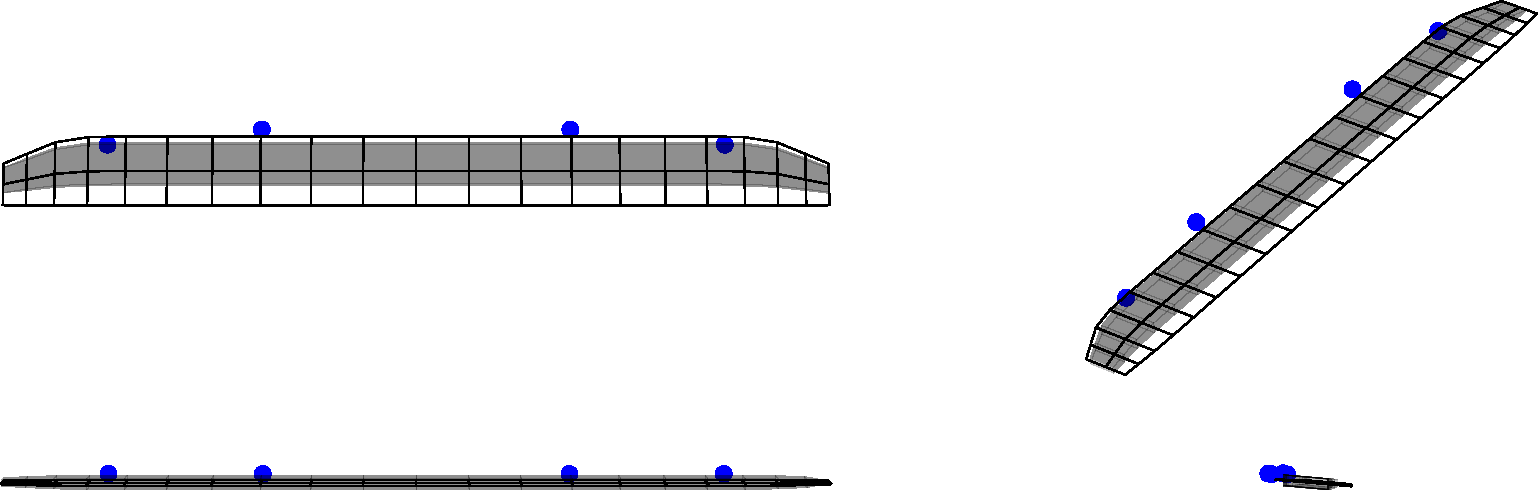
\includegraphics[width=1.0\textwidth]{../Images/aerostruct_wing}
 \caption{Three-view and isometric view of the aerostructural wing model with the engine point masses shown in blue.}
 \label{f:OAS_wing}
\end{center}
\end{figure}

We use this wing model in both the static and dynamic analyses.
For static analysis, we perform a 3-point aerostructural analysis to ensure that the internal structure of the wing does not fail during loading.
We determine the limiting loading conditions by producing a \textit{V-n} diagram, which shows the aircraft limit load factor as a function of airspeed~\cite{Raymer2012}.
This \textit{V-n} diagram is constructed using both the worst-case maneuver and gust loads to find the flight conditions where the wing structure is most likely to fail.
The \textit{V-n} diagram produced for this wing and nominal flight conditions is shown in Fig.~\ref{f:v_n_diagram}.
$V_S$ is the stall speed at normal level flight, $V_A$ is the corner speed, $V_B$ is the design speed for maximum gust intensity, $V_C$ is the design equivalent airspeed, $V_D$ is the design diving speed.
We see that the most limiting loads are at 2.8g and -1g.
Therefore, we use 1g, --1g, and 2.8g flight conditions in the 3-point aerostructural analysis in the static design.

\begin{figure}
\begin{center}
 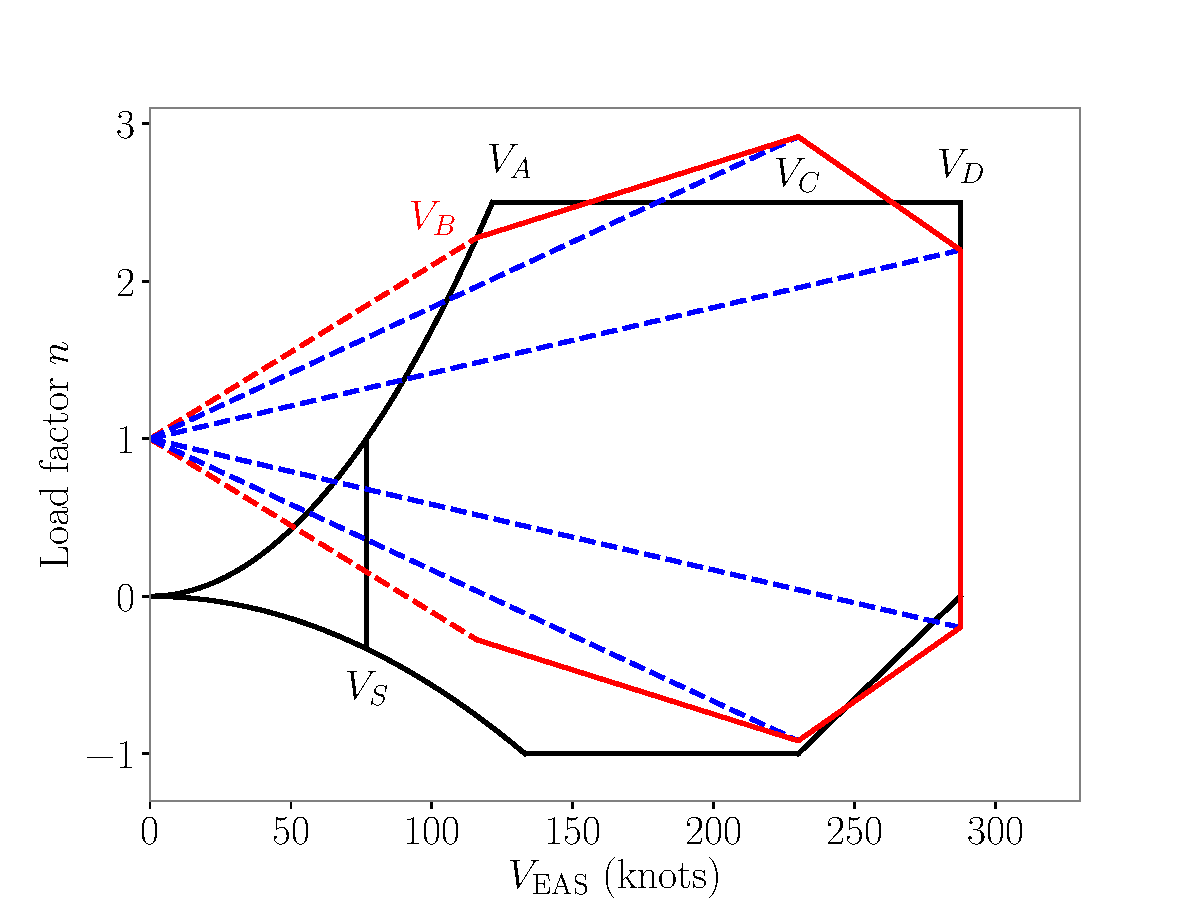
\includegraphics[width=0.6\textwidth]{../Images/v_n_diagram}
 \caption{\textit{V-n} diagram used to determine the limiting flight conditions for the wing structure.}
 \label{f:v_n_diagram}
\end{center}
\end{figure}

For the dynamic analyses, we only model the aerodynamic wing without considering the wingbox structure to lower the computational cost.
The wing deflection obtained from the 1g aerostructural analysis is applied to the wing mesh used in the aero-only cases.
Additionally, the change in results due to wing deflection across the cruise segment of the mission is negligible, which allows us to use only aerodynamic analyses in the dynamic portions of the problem.
Nominally, we will not experience structurally limiting loads during the mission, so we push the structure to the limit in the static design analysis portion.
